\chapter{Introduction}

Intro\footnotemark\\
Intro2\footnotemark\\
%note en bas de page
\iffalse
\section{Sujet}

Bla(cf. fig. 1.1)\\

%inclusion d'une mage dans le document
\begin{figure}[!h]
\begin{center}
%taille de l'image en largeur
%remplacer "width" par "height" pour régler la hauteur
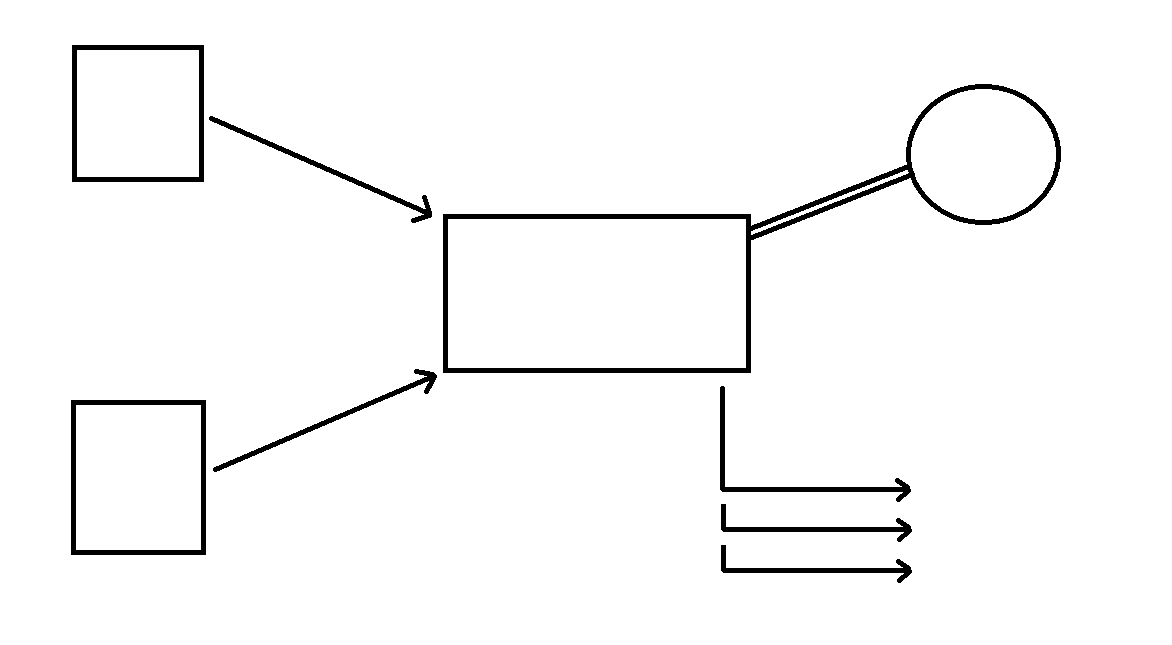
\includegraphics[width=15cm]{presentation/schema}
\end{center}
%légende de l'image
\caption{Schéma descriptif}
\end{figure}

%Contenu de la note précédemment marquée avec \footnotemark
\footnotetext{Note bas de page "intro"}

Bla
%retour à la ligne (alinea)

Bla\\
%saut de paragraphe

Bla

\newpage

\section{Problématique soulevée}

Bla

\begin{center}
Problématique du sujet
\end{center}

\section{Hypothèse de solution}

%Quoi :
Bla\\

Voici une liste :
\begin{itemize}
\item item 1;
\item item 2;
\item item 3;
\item item 4.
\end{itemize}

Bla\\

%Comment :
Bla

Bla\footnotemark\\

%Detail :
Bla(cf. ref. \cite{cite6}).
%citation référencé dans le document "bibliographie.bib" inclus à la fin du document
\fi
\footnotetext{Note bas de page "bla"}
\footnotetext{dog2}